% =====================================================================
% Paradigm Persistence as Two-Timescale Active Inference
% Fast world state s_t (real dynamics) + slow paradigm theta (belief, B~I).
% Trust figure fragments generated by _gen_trustfig.py (real graph library).
% Compile: pdflatex pomdp_paradigm_model   (inline bib; needs _trustfig_*.tex)
% =====================================================================
\documentclass[11pt,a4paper]{article}

\usepackage[T1]{fontenc}
\usepackage[utf8]{inputenc}
\usepackage[margin=1in]{geometry}
\usepackage{amsmath,amssymb,bm}
\usepackage{microtype}
\usepackage{booktabs}
\usepackage{xcolor}
\usepackage{tikz}
\usetikzlibrary{positioning,arrows.meta,calc,fit,backgrounds}
\usepackage{pgfplots}
\pgfplotsset{compat=1.18}
\usepackage[round,authoryear]{natbib}
\usepackage{hyperref}
\hypersetup{colorlinks=true,linkcolor=blue,citecolor=blue,urlcolor=blue}

\definecolor{world}{HTML}{4D4D4D}
\definecolor{paradA}{HTML}{2166AC}
\definecolor{paradB}{HTML}{B2182B}
\definecolor{social}{HTML}{1B7837}
\definecolor{util}{HTML}{D9730D}
\colorlet{adjc}{paradA}
\colorlet{trustc}{social}

\newcommand{\theory}{\theta}
\newcommand{\tstar}{\theta^{\star}}
\newcommand{\qb}{q}
\newcommand{\KL}[2]{D_{\mathrm{KL}}\!\left[#1\,\|\,#2\right]}
\newcommand{\E}[1]{\mathbb{E}\!\left[#1\right]}
\newcommand{\softmax}{\operatorname{softmax}}

\tikzset{
  lat/.style ={circle, draw=world, fill=world!8, minimum size=8mm, inner sep=1pt, font=\small},
  slow/.style={circle, draw=util, fill=util!12, minimum size=9mm, inner sep=1pt, font=\small},
  obs/.style ={circle, draw=paradA, fill=paradA!10, minimum size=8mm, inner sep=1pt, font=\small},
  anode/.style={circle, draw=paradA, fill=paradA!12, minimum size=5mm, inner sep=0pt, font=\tiny},
  chan/.style ={draw=gray!50, line width=0.4pt},
  mframe/.style={draw=gray!60, line width=0.4pt},
  >=Stealth,
}

\title{\vspace{-2.5em}Paradigm Persistence as Two-Timescale Active Inference\\[3pt]
\large A categorical POMDP with a fast world state and a slow,\\
theory-laden paradigm belief}
\author{}
\date{2026-05-21}

\begin{document}
\maketitle
\vspace{-2em}

\begin{abstract}
\noindent
Scientific communities revise theoretical commitments more slowly than the
evidence alone would dictate. We model this lag with a categorical partially
observed Markov decision process built on two latent variables operating at
separate timescales. A fast world state $s_t$, with nontrivial dynamics, is the
regime actually realised in an experiment; a slow paradigm $\theory$, with a
near-identity transition, indexes the likelihood through which observations are
read, so that the same world state yields different outcome distributions under
different paradigms. Theory-ladenness is exactly this dependence of the likelihood
on $\theory$, and the truth of a paradigm reduces to its predictive
goodness-of-fit. Inference proceeds at both timescales: the agent filters the
world state by ordinary, untempered Bayes within each paradigm, and revises its
paradigm belief by a slow, motivated variational update that trades the accuracy
of the marginal likelihood and an affective utility against a conservatism cost.
That cost---the divergence from the prior to the posterior over $\theory$---is the
informational work of re-reading the accumulated record under a new paradigm. We
embed the agent in a network, following the epistemic-communities account, in
which agents gain epistemic value from sampling like-minded neighbours, and we
take the population distribution of paradigm beliefs as the macroscopic order
parameter. With one-round transmission delays the population is a second-order
system whose approach to consensus is a damped oscillation governed by the
distribution of conservatism and the network structure; permanent lock-in is a
singular extreme. We specify the model, visualise the trust network from the graph
construction used in the implementation, and present illustrative schematics of the
target dynamics for a forthcoming numerical study.
\end{abstract}

% =====================================================================
\section{Introduction}
\label{sec:intro}
% =====================================================================

The persistence of scientific paradigms beyond the point at which evidence begins
to favour an alternative is a well-documented feature of the history of science
\citep{kuhn1962Structure,planck1949Autobiography}. A purely Bayesian agent revises
beliefs in proportion to the strength of evidence; the observed lag therefore
indicates that belief revision carries costs the cost-free Bayesian calculus omits
\citep{hylandAlbarracin2025MindChange}.

The model rests on a separation of two hidden quantities at distinct timescales. The
fast hidden state $s_t$ is the regime realised in an experiment and carries nontrivial
dynamics; the slow latent $\theory$ is the paradigm, which the agent does not sample
but maintains a belief over, and which enters the model as the likelihood through
which the world state is read. A paradigm is thus not a value of the world but a
mapping from world states to observation distributions.

This separation underlies the account that follows. Inference over the world state
is untempered and fast, whereas revision of the paradigm is slow and costly,
because changing the belief over $\theory$ alters the interpretation of every datum
already recorded. In the variational account this retroactive cost is the
complexity term of the free energy, the divergence from the prior to the posterior
over $\theory$; following \citet{hylandAlbarracin2025MindChange} we identify it
with the cost of changing one's mind. We further place the agent in a network of peers, after
\citet{albarracin2022EpistemicCommunities}, so that paradigm beliefs propagate, and
we study the population distribution of those beliefs.

Section~\ref{sec:background} reviews the components. Section~\ref{sec:model}
specifies the two-timescale generative model, the two-level inference scheme, the
trust coupling (with a visualisation of the network and its matrices from the graph
construction used in the implementation), and the regimes of slow paradigm change
the model is built to exhibit. Section~\ref{sec:anticipated} presents illustrative
schematics of the target dynamics. Section~\ref{sec:discussion} states the
layered explanation of persistence the model affords and the experimental
programme it implies.

% =====================================================================
\section{Background}
\label{sec:background}
% =====================================================================

\paragraph{Variational free energy.}
An active-inference agent maintains an approximate posterior $\qb$ over hidden
states and minimises the variational free energy of an observation $o$,
\begin{equation}
F[\qb,o]=\underbrace{-\,\E{\log p(o\mid s)}_{\qb}}_{\text{accuracy}}
        +\underbrace{\KL{\qb(s)}{p(s)}}_{\text{complexity}},
\label{eq:vfe}
\end{equation}
the sum of an accuracy term and a complexity term measuring divergence of the
posterior from the prior \citep{friston2015ActiveInferenceEpistemic}. Action is
selected to minimise expected free energy.

\paragraph{Motivated belief revision.}
\citet{hylandAlbarracin2025MindChange} reinterpret the complexity term of
Eq.~\eqref{eq:vfe} as a substantive cost of changing one's mind, and recast belief
updating as the maximisation of a belief-utility net of that cost. The
belief-utility decomposes into an affective component, independent of accuracy, and
an accuracy component; a single conservatism parameter scales the cost, ranging
from costless revision to immovable belief. The framework reproduces confirmation
bias and attitude polarisation.

\paragraph{Epistemic communities.}
\citet{albarracin2022EpistemicCommunities} model active-inference agents on a graph
who gain epistemic value from observing their neighbours' communicated beliefs; an
epistemic confirmation bias makes agents value like-minded neighbours more, driving
the formation of belief clusters.

% =====================================================================
\section{Model}
\label{sec:model}
% =====================================================================

\subsection{Two latents on two timescales}
\label{ssec:gen}

The generative model has two hidden factors. The \emph{world state}
$s_t\in\mathcal S$ is the regime realised at time $t$; it has nontrivial dynamics
$B_s(s_t\mid s_{t-1},a_{t-1})$ driven by the agent's experiment $a_{t-1}$. The
\emph{paradigm} $\theory\in\{0,\dots,K{-}1\}$ is a slow latent with a
near-identity transition $B_\theory\approx I$; it is not resampled but inferred.
The model factorises as
\begin{equation}
p(o_{1:T},s_{1:T},\theory)
= p(\theory)\prod_{t} p(o_t\mid s_t,\theory)\,
   p(s_t\mid s_{t-1},a_{t-1}) ,
\label{eq:gen}
\end{equation}
and the agent's posterior factorises accordingly,
$q(s_{1:T},\theory)=q(\theory)\prod_t q(s_t\mid\theory)$. The separation of
timescales is the defining feature of the model: the world state evolves quickly
and the paradigm slowly, and the agent infers both.
Figure~\ref{fig:factor} shows the structure.

\begin{figure}[t]
\centering
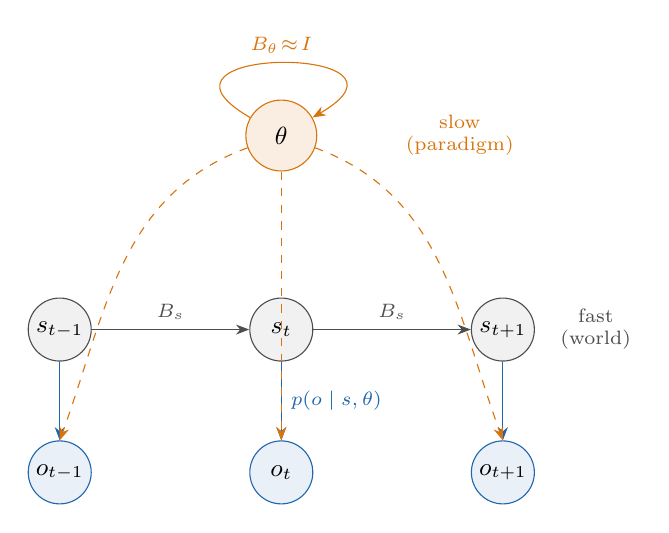
\begin{tikzpicture}[node distance=12mm]
\node[slow] (th) {$\theory$};
\node[lat] (s2) [below=16mm of th] {$s_t$};
\node[lat] (s1) [left=20mm of s2] {$s_{t-1}$};
\node[lat] (s3) [right=20mm of s2] {$s_{t+1}$};
\node[obs] (o1) [below=10mm of s1] {$o_{t-1}$};
\node[obs] (o2) [below=10mm of s2] {$o_{t}$};
\node[obs] (o3) [below=10mm of s3] {$o_{t+1}$};
% fast chain
\draw[->,world] (s1) -- node[above,font=\scriptsize]{$B_s$} (s2);
\draw[->,world] (s2) -- node[above,font=\scriptsize]{$B_s$} (s3);
% likelihoods
\draw[->,paradA] (s1) -- (o1);
\draw[->,paradA] (s2) -- node[right,font=\scriptsize]{$p(o\mid s,\theory)$} (o2);
\draw[->,paradA] (s3) -- (o3);
% theta reads every observation
\draw[->,util,dashed] (th) to[out=200,in=70] (o1.north);
\draw[->,util,dashed] (th) -- (o2.north);
\draw[->,util,dashed] (th) to[out=-20,in=110] (o3.north);
% near-identity slow transition
\draw[->,util] (th) to[out=150,in=30,looseness=6] node[above,font=\scriptsize]{$B_\theory\!\approx\! I$} (th);
\node[font=\scriptsize, world, align=center] at (s3.east) [right=2mm] {fast\\(world)};
\node[font=\scriptsize, util, align=center] at (th.east) [right=10mm] {slow\\(paradigm)};
\end{tikzpicture}
\caption{The two-timescale generative model. The world state $s_t$ (grey) evolves
under nontrivial dynamics $B_s$ and emits observations through the likelihood
$p(o_t\mid s_t,\theory)$ (blue). The paradigm $\theory$ (orange) is a slow latent
($B_\theory\approx I$) that conditions every likelihood (dashed): it does not move
the world, it sets how the world is read. The agent infers both factors.}
\label{fig:factor}
\end{figure}

\subsection{Theory-laden likelihood}
\label{ssec:like}

For each paradigm $\theory$ and world state $s$, the likelihood
$p(o\mid s,\theory)$ is a categorical distribution over a finite outcome set
$\mathcal O$. Theory-ladenness is the dependence of this distribution on $\theory$:
the same world state $s$ produces different outcome distributions read through
different paradigms, so no two paradigms interpret a datum identically. We make no
metaphysical claim that the world possesses a true paradigm. The world generates
observations through some $\tstar$, which need not lie in the agent's hypothesis
set; the agent maintains a posterior over which $\theory$ best predicts its
experience, and the question ``which paradigm is true'' reduces to predictive
goodness-of-fit. The capacity of an experiment to discriminate paradigms,
\begin{equation}
d(a)=\tfrac12\!\sum_{\theory\neq\theory'}\!
   \KL{p(o\mid s,\theory)}{p(o\mid s,\theory')},
\label{eq:discrim}
\end{equation}
is small when paradigms predict similar outcomes (the experiment is
underdetermined) and large when they predict different ones.

\subsection{Two-level inference}
\label{ssec:infer}

Both latents are revised by the \emph{same} update---the motivated belief-utility
maximisation of \citet{hylandAlbarracin2025MindChange}---and the two timescales are
two settings of its parameters, not two mechanisms. For a belief $\qb$ over a latent
with carried-over prior $q_0$ and evidence summarised by a marginal likelihood $L$,
\begin{equation}
q'=\arg\max_{\qb}\Bigl\{\,U[\qb]+\alpha\,\E{\log L}_{\qb}-\lambda\,\KL{\qb}{q_0}\,\Bigr\}
\qquad\Longrightarrow\qquad
q'\;\propto\;q_0\,L^{\alpha/\lambda}\,e^{\,u/\lambda},
\label{eq:motiv}
\end{equation}
a tempered Bayesian rule with effective learning rate $\alpha/\lambda$: the accuracy
weight $\alpha$ scales the pull of the evidence, the conservatism $\lambda$ the cost
of moving, and the affective utility $u$ (with $U[\qb]=\E{u}_{\qb}$) a preference
over which value is believed, independent of fit. Ordinary Bayes is the corner
$\alpha=\lambda$, $u=0$, where the learning rate is one and the prior is updated by
the likelihood alone.

\paragraph{Fast: untempered filtering of the world state.}
The world state sits at that corner. Its prior is the one-step prediction
$\sum_{s_{t-1}}B_s(s_t\mid s_{t-1},a_{t-1})\,q(s_{t-1}\mid\theory)$---present because
$B_s$ has nontrivial dynamics---and at $\alpha=\lambda$, $u=0$ Eq.~\eqref{eq:motiv}
collapses to the exact Bayes filter
\begin{equation}
q(s_t\mid\theory)\;\propto\;p(o_t\mid s_t,\theory)
   \sum_{s_{t-1}} B_s(s_t\mid s_{t-1},a_{t-1})\,q(s_{t-1}\mid\theory).
\label{eq:fast}
\end{equation}
The world state carries no conservatism because there is no standing commitment to
resist revising: the regime is expected to change at every step, so tracking it
responsively is correct, not motivated.

\paragraph{Slow: motivated revision of the paradigm.}
The paradigm sits away from the corner, with $\alpha<\lambda$ and possibly
$u(\theory)\neq0$. Its prior is the carried-over belief $q(\theory)$---there is no
prediction step, since $B_\theory\approx I$---and the evidence is the marginal
likelihood each paradigm assigns the new datum,
\begin{equation}
L(\theory\mid o_t)=\sum_{s_t} p(o_t\mid s_t,\theory)\,q(s_t\mid\theory).
\label{eq:marglik}
\end{equation}
Instantiating Eq.~\eqref{eq:motiv} gives the paradigm update
\begin{equation}
q'(\theory)=\arg\max_{\qb}\Bigl\{\,U[\qb]+\alpha\,\E{\log L(\theory\mid o_t)}_{\qb}
   -\lambda\,\KL{\qb}{q(\theory)}\,\Bigr\}
\;\propto\;q(\theory)\,L(\theory\mid o_t)^{\alpha/\lambda}\,e^{\,u(\theory)/\lambda}.
\label{eq:slow}
\end{equation}
The asymmetry between the factors is therefore a choice of \emph{where} conservatism
applies, not a second kind of inference: the world state is tracked responsively
because it moves, while the paradigm---a near-static commitment---is revised only as
fast as its cost permits.

\paragraph{Conservatism as an institutional-memory cost.}
What does the conservatism $\lambda$ encode? As written in
\citet{hylandAlbarracin2025MindChange}, the cost is the one-step divergence
$\KL{q'(\theory)}{q(\theory)}$ between successive paradigm posteriors---the immediate
effort of moving one's belief now. We read its magnitude as a proxy for a larger,
retroactive operation. Because $\theory$ conditions the likelihood of every past
datum (Eq.~\ref{eq:gen}), adopting a new paradigm means re-reading the entire
accumulated record under a new likelihood. For a single agent this is the cost of
recomputing how all prior observations should now be understood; for a community it
is an \emph{institutional-memory} cost---textbooks, curricula, calibrated
instruments, and accepted exemplars are encodings of the prevailing $\theory$, and a
paradigm shift devalues that shared capital and forces its reconstruction. We are
explicit that this archive-recoding reading is an interpretation we place on
$\lambda$, not a separate term in the objective: Eq.~\eqref{eq:slow} computes only
the one-step KL, and we take its size to stand in for the retroactive work, with
larger $\lambda$ marking paradigms whose record is more expensive to recode. So read,
$\lambda$ supplies a formal counterpart of incommensurability---resistance to
paradigm change as the informational cost of re-interpreting the past, not a
departure from rationality---while we note that a literal accounting of that cost
would sum over the history rather than compare two adjacent posteriors.

\subsection{Policy and selective attention}
\label{ssec:policy}

Experiments are selected by expected free energy
\citep{friston2015ActiveInferenceEpistemic}. The data that move $q(\theory)$ are
the discriminating ones---outcomes improbable under every world state for the
current paradigm---and these are exactly the experiments a confirmation-biased
policy avoids. This bias arises in two equivalent ways: through the epistemic
confirmation bias $\gamma$ of \citet{albarracin2022EpistemicCommunities}, and
through a small affective utility $u(\theory)$ tilting the planning belief, so that
discriminating experiments appear risky to the preferred paradigm and are
under-sampled.

\subsection{Trust and the social network}
\label{ssec:trust}

The agent is one of $N$ on a graph $\mathcal G=(V,E)$, each carrying its own
$\bigl(q_i(s_t\mid\theory),\,q_i(\theory),\,\lambda_i,\,U_i\bigr)$. Each agent emits
its paradigm belief, and agent $i$ forms a social observation as the trust-weighted
mixture of its neighbours' emissions, $o^{\mathrm s}_i=\sum_j T_{ij}\,q_j(\theory)$,
where $T$ is the row-stochastic \emph{trust matrix}, constructed from the graph
adjacency $A$ by row normalisation, $T=\mathrm{rownorm}(A)$. The matrix carries no
self term: an agent's reliance on its own current belief is already represented by
the prior in the slow update~\eqref{eq:slow}, weighted against incoming evidence by
the conservatism $\lambda$, so a self-weight in $T$ would duplicate that inertia.
The trust matrix therefore encodes only which neighbours an agent attends to, a role
distinct from $\lambda$; the strength of the social channel is set by a message
precision $\kappa$, and the confirmation bias $\gamma$ up-weights aligned
neighbours. The social signal enters the slow update~\eqref{eq:slow} as a second
accuracy channel. Figure~\ref{fig:trust} shows a Watts--Strogatz instance, its
adjacency $A$, and the induced trust matrix $T$ from the graph construction used in
the implementation. The macroscopic object of interest is the \emph{distribution} of
the paradigm beliefs $\{q_i(\theory)\}$ across the population.

\begin{figure}[t]
\centering
\begin{minipage}[b]{0.35\textwidth}\centering
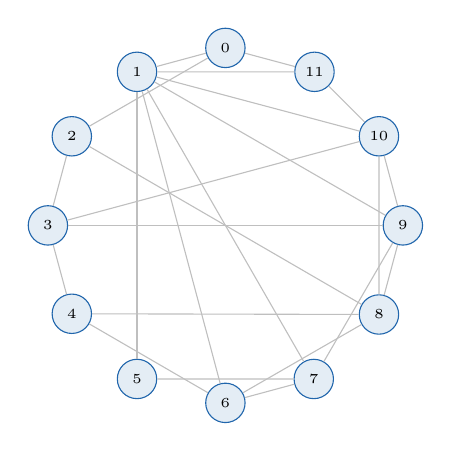
\begin{tikzpicture}[scale=0.92]
\node[anode] (n0) at (0.00,2.45) {0};
\node[anode] (n1) at (-1.22,2.12) {1};
\node[anode] (n2) at (-2.12,1.23) {2};
\node[anode] (n3) at (-2.45,0.00) {3};
\node[anode] (n4) at (-2.12,-1.22) {4};
\node[anode] (n5) at (-1.22,-2.12) {5};
\node[anode] (n6) at (-0.00,-2.45) {6};
\node[anode] (n7) at (1.22,-2.12) {7};
\node[anode] (n8) at (2.12,-1.23) {8};
\node[anode] (n9) at (2.45,-0.00) {9};
\node[anode] (n10) at (2.12,1.23) {10};
\node[anode] (n11) at (1.23,2.12) {11};
\draw[chan] (n0) -- (n1);
\draw[chan] (n0) -- (n2);
\draw[chan] (n0) -- (n11);
\draw[chan] (n1) -- (n5);
\draw[chan] (n1) -- (n6);
\draw[chan] (n1) -- (n7);
\draw[chan] (n1) -- (n9);
\draw[chan] (n1) -- (n10);
\draw[chan] (n1) -- (n11);
\draw[chan] (n2) -- (n3);
\draw[chan] (n2) -- (n8);
\draw[chan] (n3) -- (n4);
\draw[chan] (n3) -- (n9);
\draw[chan] (n3) -- (n10);
\draw[chan] (n4) -- (n6);
\draw[chan] (n4) -- (n8);
\draw[chan] (n5) -- (n7);
\draw[chan] (n6) -- (n7);
\draw[chan] (n6) -- (n8);
\draw[chan] (n7) -- (n9);
\draw[chan] (n8) -- (n9);
\draw[chan] (n8) -- (n10);
\draw[chan] (n9) -- (n10);
\draw[chan] (n10) -- (n11);

\end{tikzpicture}\\[2pt]
{\footnotesize (a) agents and channels}
\end{minipage}\hfill
\begin{minipage}[b]{0.31\textwidth}\centering
\begin{tikzpicture}
\input{_trustfig_adj}
\node[font=\scriptsize] at (2.04,0.65) {$j$};
\node[font=\scriptsize,rotate=90] at (-0.45,-1.7) {$i$};
\end{tikzpicture}\\[2pt]
{\footnotesize (b) adjacency $A$}
\end{minipage}\hfill
\begin{minipage}[b]{0.31\textwidth}\centering
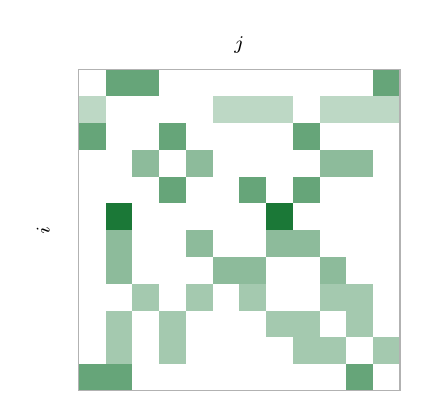
\begin{tikzpicture}
\fill[trustc!67] (0.340,0.000) rectangle (0.680,0.340);
\fill[trustc!67] (0.680,0.000) rectangle (1.020,0.340);
\fill[trustc!67] (3.740,0.000) rectangle (4.080,0.340);
\fill[trustc!29] (0.000,-0.340) rectangle (0.340,0.000);
\fill[trustc!29] (1.700,-0.340) rectangle (2.040,0.000);
\fill[trustc!29] (2.040,-0.340) rectangle (2.380,0.000);
\fill[trustc!29] (2.380,-0.340) rectangle (2.720,0.000);
\fill[trustc!29] (3.060,-0.340) rectangle (3.400,0.000);
\fill[trustc!29] (3.400,-0.340) rectangle (3.740,0.000);
\fill[trustc!29] (3.740,-0.340) rectangle (4.080,0.000);
\fill[trustc!67] (0.000,-0.680) rectangle (0.340,-0.340);
\fill[trustc!67] (1.020,-0.680) rectangle (1.360,-0.340);
\fill[trustc!67] (2.720,-0.680) rectangle (3.060,-0.340);
\fill[trustc!50] (0.680,-1.020) rectangle (1.020,-0.680);
\fill[trustc!50] (1.360,-1.020) rectangle (1.700,-0.680);
\fill[trustc!50] (3.060,-1.020) rectangle (3.400,-0.680);
\fill[trustc!50] (3.400,-1.020) rectangle (3.740,-0.680);
\fill[trustc!67] (1.020,-1.360) rectangle (1.360,-1.020);
\fill[trustc!67] (2.040,-1.360) rectangle (2.380,-1.020);
\fill[trustc!67] (2.720,-1.360) rectangle (3.060,-1.020);
\fill[trustc!100] (0.340,-1.700) rectangle (0.680,-1.360);
\fill[trustc!100] (2.380,-1.700) rectangle (2.720,-1.360);
\fill[trustc!50] (0.340,-2.040) rectangle (0.680,-1.700);
\fill[trustc!50] (1.360,-2.040) rectangle (1.700,-1.700);
\fill[trustc!50] (2.380,-2.040) rectangle (2.720,-1.700);
\fill[trustc!50] (2.720,-2.040) rectangle (3.060,-1.700);
\fill[trustc!50] (0.340,-2.380) rectangle (0.680,-2.040);
\fill[trustc!50] (1.700,-2.380) rectangle (2.040,-2.040);
\fill[trustc!50] (2.040,-2.380) rectangle (2.380,-2.040);
\fill[trustc!50] (3.060,-2.380) rectangle (3.400,-2.040);
\fill[trustc!40] (0.680,-2.720) rectangle (1.020,-2.380);
\fill[trustc!40] (1.360,-2.720) rectangle (1.700,-2.380);
\fill[trustc!40] (2.040,-2.720) rectangle (2.380,-2.380);
\fill[trustc!40] (3.060,-2.720) rectangle (3.400,-2.380);
\fill[trustc!40] (3.400,-2.720) rectangle (3.740,-2.380);
\fill[trustc!40] (0.340,-3.060) rectangle (0.680,-2.720);
\fill[trustc!40] (1.020,-3.060) rectangle (1.360,-2.720);
\fill[trustc!40] (2.380,-3.060) rectangle (2.720,-2.720);
\fill[trustc!40] (2.720,-3.060) rectangle (3.060,-2.720);
\fill[trustc!40] (3.400,-3.060) rectangle (3.740,-2.720);
\fill[trustc!40] (0.340,-3.400) rectangle (0.680,-3.060);
\fill[trustc!40] (1.020,-3.400) rectangle (1.360,-3.060);
\fill[trustc!40] (2.720,-3.400) rectangle (3.060,-3.060);
\fill[trustc!40] (3.060,-3.400) rectangle (3.400,-3.060);
\fill[trustc!40] (3.740,-3.400) rectangle (4.080,-3.060);
\fill[trustc!67] (0.000,-3.740) rectangle (0.340,-3.400);
\fill[trustc!67] (0.340,-3.740) rectangle (0.680,-3.400);
\fill[trustc!67] (3.400,-3.740) rectangle (3.740,-3.400);
\draw[mframe] (0,0.340) rectangle (4.080,-3.740);

\node[font=\scriptsize] at (2.04,0.65) {$j$};
\node[font=\scriptsize,rotate=90] at (-0.45,-1.7) {$i$};
\end{tikzpicture}\\[2pt]
{\footnotesize (c) trust / update matrix $T$}
\end{minipage}
\caption{The trust network, from the Watts--Strogatz construction
($N{=}12$, $k{=}4$, rewiring $0.25$) used in the implementation. (a)~Agents
(nodes) and their communication channels (edges). (b)~The binary adjacency matrix
$A$: a filled cell at $(i,j)$ marks a channel. (c)~The row-stochastic trust matrix
$T=\mathrm{rownorm}(A)$, whose row $i$ gives the weights with which agent $i$ mixes
its neighbours' paradigm beliefs into its social observation; darker cells carry
more weight, and the diagonal is empty because own-belief inertia is supplied by the
conservatism $\lambda$, not by $T$. Iterating the update propagates beliefs along
these channels.}
\label{fig:trust}
\end{figure}

\subsection{Regimes of slow paradigm change}
\label{ssec:regimes}

The model makes the slowness of paradigm change a consequence of four distinct,
separately measurable causes, three at the level of the individual and one social:
\begin{enumerate}\setlength{\itemsep}{2pt}
\item \textbf{Conservatism} $\lambda$ large---the archive-recoding cost of
  Eq.~\eqref{eq:slow} makes the paradigm update slow even when evidence is decisive.
\item \textbf{Structural ambiguity}---small marginal-likelihood ratios, i.e.\ low
  discriminability $d(a)$ (Eq.~\ref{eq:discrim}); the world does not separate the
  paradigms.
\item \textbf{Selective attention}---a policy biased away from discriminating
  experiments (Section~\ref{ssec:policy}), so the sharpening data are not gathered.
\item \textbf{Social inertia}---neighbours have not moved either, so the social
  channel pulls back toward the prevailing paradigm.
\end{enumerate}
Each can produce the appearance of a stuck community without any individual being
unreasonable. The extreme limits---$\lambda\to\infty$, or an affective utility that
overpowers the accuracy term---yield permanent lock-in, but these are singular; for
finite conservatism and adequate discriminating evidence the paradigm belief still
moves, and the population converges. The phenomenon to be characterised is therefore
not lock-in but the \emph{transient}.

% =====================================================================
\section{Anticipated results}
\label{sec:anticipated}
% =====================================================================

The curves below are illustrative schematics, not simulation output; they specify
the target phenomenology a numerical study of the model is intended to produce. The
macroscopic variable is the population's marginal paradigm belief. With one-round
transmission delays through the graph (Section~\ref{ssec:trust}), the coupled
population is a second-order system, and its approach to consensus is a damped
oscillation whose damping ratio is set by the distribution of conservatism
$\{\lambda_i\}$ and by the spectral structure of $T$. Figure~\ref{fig:anticipated}(a)
shows the family of damping regimes the model should exhibit; panel~(b) shows the
individual-level belief trajectories distinguishing convergence from the two lock-in
extremes.

\begin{figure}[t]
\centering
\begin{minipage}{0.49\textwidth}\centering
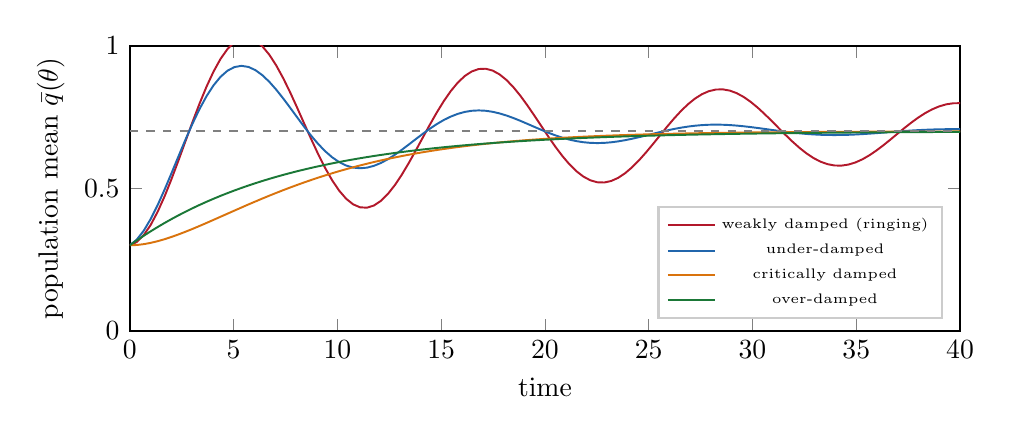
\begin{tikzpicture}
\begin{axis}[width=\textwidth,height=5.2cm,
  xlabel={time}, ylabel={population mean $\bar q(\theory)$},
  xmin=0,xmax=40,ymin=0,ymax=1,ytick={0,0.5,1},
  legend style={font=\tiny,at={(0.98,0.04)},anchor=south east,draw=gray!40},
  domain=0:40,samples=120,thick,every axis plot/.append style={line width=0.7pt}]
\addplot[paradB]{0.7-0.4*exp(-0.035*x)*cos(deg(0.55*x))};
\addlegendentry{weakly damped (ringing)}
\addplot[paradA]{0.7-0.4*exp(-0.10*x)*cos(deg(0.55*x))};
\addlegendentry{under-damped}
\addplot[util]{0.7-0.4*exp(-0.22*x)*(1+0.22*x)};
\addlegendentry{critically damped}
\addplot[social]{0.7-0.4*exp(-0.13*x)};
\addlegendentry{over-damped}
\draw[gray,dashed] (axis cs:0,0.7)--(axis cs:40,0.7);
\end{axis}
\end{tikzpicture}\\[2pt]
{\footnotesize (a) damped-oscillation regimes vs.\ conservatism distribution}
\end{minipage}\hfill
\begin{minipage}{0.49\textwidth}\centering
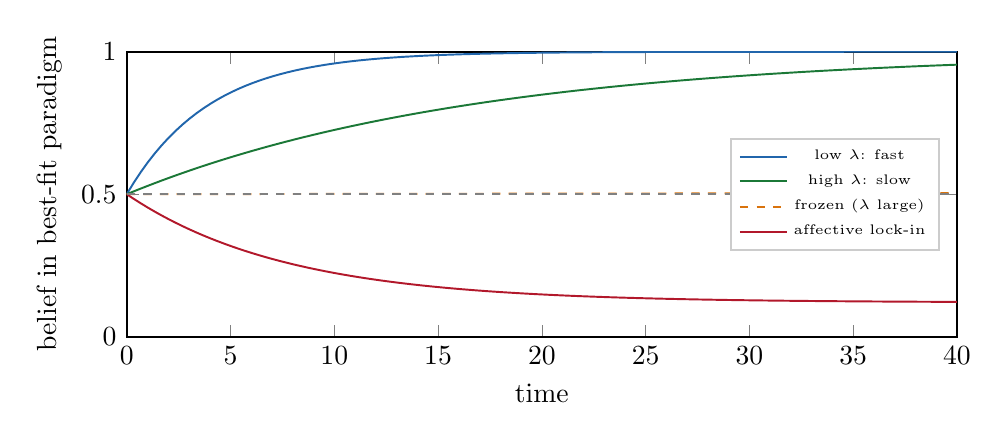
\begin{tikzpicture}
\begin{axis}[width=\textwidth,height=5.2cm,
  xlabel={time}, ylabel={belief in best-fit paradigm},
  xmin=0,xmax=40,ymin=0,ymax=1,ytick={0,0.5,1},
  legend style={font=\tiny,at={(0.98,0.5)},anchor=east,draw=gray!40},
  domain=0:40,samples=120,thick,every axis plot/.append style={line width=0.7pt}]
\addplot[paradA]{1-0.5*exp(-0.25*x)};
\addlegendentry{low $\lambda$: fast}
\addplot[social]{1-0.5*exp(-0.06*x)};
\addlegendentry{high $\lambda$: slow}
\addplot[util,dashed]{0.5+0.0001*x};
\addlegendentry{frozen ($\lambda$ large)}
\addplot[paradB]{0.12+0.38*exp(-0.13*x)};
\addlegendentry{affective lock-in}
\draw[gray,dashed] (axis cs:0,0.5)--(axis cs:40,0.5);
\end{axis}
\end{tikzpicture}\\[2pt]
{\footnotesize (b) individual regimes: convergence vs.\ lock-in}
\end{minipage}
\caption{Illustrative target dynamics (schematic; not simulation output).
(a)~The population's mean paradigm belief approaches consensus (dashed line) as a
damped oscillation; the damping regime---weakly damped ringing, under-damped,
critically damped, over-damped---is set by the distribution of conservatism
$\{\lambda_i\}$ and the network structure. (b)~At the individual level, finite
conservatism yields convergence to the best-fit paradigm (fast or slow). All
trajectories start from a neutral belief: under unbounded conservatism the belief
stays frozen at its prior, while a supra-threshold affective utility pulls the
belief toward the preferred non-best-fit paradigm, so belief in the best-fit
paradigm declines toward a low fixed point.}
\label{fig:anticipated}
\end{figure}

% =====================================================================
\section{Discussion}
\label{sec:discussion}
% =====================================================================

The two-timescale construction yields a layered answer to why communities do not
switch paradigms when the evidence turns. The marginal likelihood favouring an
alternative is often small because the world is structurally ambiguous; the policy
does not seek the experiments that would sharpen it because attention is tilted by
preference; even when discriminating evidence arrives, the cost of re-coding the
accumulated record makes the paradigm update slow; and neighbours have not moved
either. Four causes, four timescales, one model. None requires an agent to be
irrational: each agent performs exact Bayesian inference over the world state and
revises its theory at a rate its costs justify.

Two features distinguish the account. First, separating the fast world state from
the slow paradigm locates theory-ladenness in a single
interpretable place, the dependence of the likelihood on $\theory$. Second,
identifying the conservatism cost with the informational work of re-coding the
archive gives a formal counterpart of incommensurability and grounds Hyland's cost
of mind-change in the retroactive reach of a paradigm over past data.

The model implies a concrete programme. The primary independent variable is the
population distribution of conservatism $\{\lambda_i\}$; secondary variables are the
experimental discriminability $d(a)$, the affective-utility distribution $\{U_i\}$,
and the social coupling encoded in $T$, $\kappa$, and $\gamma$. The primary
dependent variable is the damping of the population's approach to consensus, with
the time to consensus and the incidence of lock-in as derived quantities. The model
predicts that lock-in does not occur for finite conservatism and sub-threshold
affective utility regardless of social coupling, which is a falsifiable boundary,
and that the qualitative dynamics are governed by the conservatism distribution
rather than by any single agent's parameters.

% =====================================================================
\section{Conclusion}
\label{sec:conclusion}
% =====================================================================

We have presented a categorical POMDP of paradigm persistence built on two latents
at separate timescales: a fast world state with nontrivial dynamics and a slow,
theory-laden paradigm maintained as a belief. World-state inference is exact,
untempered Bayes; paradigm inference is a slow, motivated, tempered update whose
conservatism cost is the work of re-coding the accumulated record. Networked agents propagate
paradigm beliefs through a trust matrix, and the population's distribution of
paradigm beliefs approaches consensus as a damped oscillation set by the
distribution of conservatism. The model converts the question of permanent capture
into a question about the damping of convergence and identifies the distribution of
resistance to changing one's mind as the variable that controls it.

\begin{thebibliography}{9}
\bibitem[Albarracin et al.(2022)]{albarracin2022EpistemicCommunities}
M.~Albarracin, D.~Demekas, M.~J.~D.~Ramstead, and C.~Heins.
\newblock Epistemic Communities under Active Inference.
\newblock \emph{Entropy}, 24(4):476, 2022.

\bibitem[Friston et al.(2015)]{friston2015ActiveInferenceEpistemic}
K.~Friston, F.~Rigoli, D.~Ognibene, C.~Mathys, T.~Fitzgerald, and G.~Pezzulo.
\newblock Active inference and epistemic value.
\newblock \emph{Cognitive Neuroscience}, 6(4):187--214, 2015.

\bibitem[Hyland and Albarracin(2025)]{hylandAlbarracin2025MindChange}
D.~Hyland and M.~Albarracin.
\newblock On the Variational Costs of Changing Our Minds.
\newblock \emph{arXiv preprint} arXiv:2509.17957, 2025.

\bibitem[Kuhn(1962)]{kuhn1962Structure}
T.~S.~Kuhn.
\newblock \emph{The Structure of Scientific Revolutions}.
\newblock University of Chicago Press, 1962.

\bibitem[Planck(1949)]{planck1949Autobiography}
M.~Planck.
\newblock \emph{Scientific Autobiography and Other Papers}.
\newblock Philosophical Library, 1949.
\end{thebibliography}

\end{document}
